\documentclass[a4paper,11pt]{article}

%\setlength{\headheight}{22.62503pt}

% Use packages to set margins, fonts, and spacing
\usepackage[margin=2.5cm,headheight=22.28003pt,top=2.5cm]{geometry}
\usepackage{amssymb}
\usepackage{mathptmx}
\usepackage{setspace}
\usepackage{amsmath}
\usepackage{mathptmx}
\usepackage{graphicx}
\usepackage{lipsum} % this package is used to create dummy text.
\usepackage{enumitem}

\usepackage[utf8]{inputenc}


\usepackage{graphicx}
\usepackage{lipsum}

\newcommand{\coversection}[2]{
  \newpage
  \thispagestyle{empty}
  \begin{center}
    \vspace*{\fill}
    \includegraphics[width=0.5\linewidth]{#1}
    \vspace*{0.5cm} % Anpassung des Abstands
    \par
    \Large\textbf{#2}
    \par\vspace{\fill}
  \end{center}
  \newpage
}




\begin{document}
\coversection{turing.png}{Turingmachine}
\section*{Berechenbarkeit}
\section{Turingmachine} 
\begin{sloppypar}
  Wir Betrachte das folgende, sehr bekannt, berechnunsmodell. Anschaulich lässt es sich wie folht beschreiben.
\end{sloppypar} 
\begin{itemize}
  \renewcommand\labelitemi{-}
  \item Es gibt einen "Speicher" $\leadsto $ k unendlich lange Arrays(\textbf{Bänder})
  \item Es gibt einen "Arbeitsspeicher" $\leadsto$ eine endliche Menge von Zusänden, die die Machine einnehmen kann
  \item Für jedes Band gibt es einen Schreib- und Lesekopf 
  \item Jeder Schritt ist wie folgt:\\ Abhängig von Zustand und gelesenene Symbol, Schreiben die Küpfe genau ein Symbol, bewegen sich nun maximal eine Position und der Zustand der Machine wird geändert.
  \item Stellt die Machine ihhr schrittweises Arbeiten ein, so wird die Ausgabe entweder den Zustand entnommen oder von einem der Bänder in geeigneter Weise abgelesen.
\end{itemize}

\begin{figure}[htp]
  \centering
  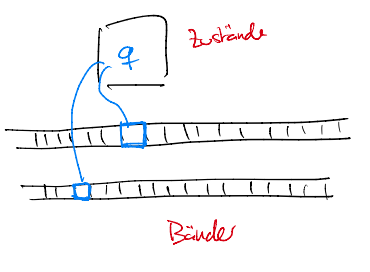
\includegraphics[width=0.5\textwidth]{turing_sym.png}
  \caption{Turingmachine.}
  \label{fig:tm}
\end{figure}

\subsection{Definition (Turingmachine, Alan Tuing, 1936)} Sei $k \in \mathbb{N}$ eine \textbf{k-Band-Turingmachine}m kurz k-TM, ist ein Tupe $M = (Q, \Sigma, \varGamma, \Delta, s, F )$. Dabei ist:
\begin{itemize}
  \item Q eine endliche Menge, \textbf{Zustandmenge}
  \item $\Sigma$ das \textbf{Eingabealphabet}, ein Alphabet $\Box \not \in \Sigma$
  \item $\varGamma$ das \textbf{Bandaphabet}, ein Alphabet mit $\Sigma \subseteq \varGamma$ und $\Box \in \varGamma / \Sigma$ 
  \item $\Delta \subseteq Q \times \varGamma^{k} \rightarrow \subseteq Q \times \varGamma^{k} \times {L, S, R}^{k}$ die \textbf{Übergangsrelation}
  \item $s \in Q$ der \textbf{Startzustand}
  \item $F \subseteq Q$ die Menge der \textbf{akzeptierenden Zustände} 
\end{itemize}
\begin{sloppypar}
  \noindent Das Symbol $\Box$ heißt \textbf{Blank}. Die Elemente von $\Delta$ heißen \textbf{instruktionen}. Für eine Instruktion $(q_{1}, a_{1}, \cdots, a_{k}, q', a'_{1}, \cdots, a'_{k}, B_{1}, \cdots, B_{k})$ \textbf{Anweisungteil}. Die TM M ist eine \textbf{deterministische k-Band Turingmachine}, kurz k-DTM, wenn es $\forall b \in Q \times \varGamma^{k}$ höchstens eine Instruktion $i \in \Delta$ mit Bedingungsteil b.
\end{sloppypar}

\subsection{Definition (Konfiguration)} Sei $M = (Q, \Sigma, \Gamma, \Delta, s, F)$ eine k-TM. EIne \textbf{Konfigration} von M ist ein Tupel \[C = (q, w_{1}, \cdots, w_{k}, p_{1}, \cdots, p_{k}) \in Q \times (p^{*})^{k} \times \mathbb{N}^{k}\] Die \textbf{Startkonfiguration} von M zur Eingabe $(u_{1}, \cdots, u_{n}) \in (\Sigma^{*})^{n}$, wobei $n \in \mathbb{N}$, ist die Konfiguration \[Start_{M}(u_{1}, \cdots, u_{n}) = (s, u_{1} \Box u_{2} \Box \cdots \Box u_{n}, \Box, \cdots, 1, \cdots, 1)\] Die Konfiguration C ist eine \textbf{Stoppkonfigration} von M, wenn es keine Instruktion $i \in \Delta$ mit Bedingungsteil $(q, w_{1}(p_{1}), \cdots, w_{k}(p_{k}))$ gibt.

\subsection{Definition (Nachfolgekonfiguration)}
\end{document}
